\chapter{提案手法}
\label{chap:proposal}
\ref{sec:rlto2048}節で述べたように, 2048を対象とした強化学習の研究は数多くなされてきた.
もしゲームが完全に解かれていれば, 強化学習手法の良し悪しを定量的に評価することができる.
一方で2048はゲーム木の大きさから, 完全解析を実行することは計算資源の観点から困難である.
そこで本研究では2048のミニゲームの完全解析を行うことを提案する.
さらに解析したミニゲームをベンチマークとして, 2048の強化学習手法について詳細に検討する.

\section{2048のミニゲームの完全解析}
\label{chap:solving}
\ref{chap:rl}章で述べた強化学習は環境~(ゲーム)~と何度もやり取りすることで, 最適な方策を学習するための手法である.
一方で小さなゲームであれば, 力ずくの計算によってゲームを完全に解くこともできる.
本章では2048を解析的なアプローチによって解くことについて考察する.

\subsection{2048の完全解析とは}
\label{sec:solving}
2048は$1$人用のゲームであるため, 勝敗のようなプレイヤの明確な目標は存在しない.
そのためプレイヤが何を目標とするかによって, プレイヤの最善手の定義は変化する.
また\ref{sec:rule}節で述べたようにゲームはランダム性を伴うため, 同じ状態から毎回同じ手を選んでも結果は確率的に変動する.

そこで本稿ではある状態$s$における最善手を「$s$から獲得できる得点の合計の期待値が最も高くなるような手」と定義する.
これは~\ref{chap:rl}節で述べた強化学習の最適状態価値と等価なものである.
よって状態$s$から最善手を選び続けて獲得できる得点の合計の期待値を状態$s$の最適価値と呼び, $v_*(s)$で表すことにする.

このとき$v_*(s)$は式~\ref{eq:value}のように再帰的な形式で書くことができる.
\begin{align}
    v_*(s) =
    \begin{cases}
        0 & (s \text{が終了状態}) \\
        \max_a \left(r(s,a) + \mathbb{E}_{s_\text{next} \in \mathcal{T}(s,a)} v_*(s_\text{next}) \right) & (\text{otherwise})
    \end{cases}
    \label{eq:value}
\end{align}
ただし$r(s,a)$は状態$s$から行動$a$をとって獲得する得点, $s_\text{next} \in \mathcal{T}(s,a)$は状態$s$から行動$a$をとって遷移しうる次の状態の集合を表す~(図~\ref{fig:state_afterstate}を参照).
式~\ref{eq:value}の$r(s,a) + \mathbb{E}_{s_\text{next} \in \mathcal{T}(s,a)} v_*(s_\text{next})$は, 強化学習における最適行動価値$q_*(s,a)$に対応する.
また$\mathbb{E}_{s_\text{next} \in \mathcal{T}(s,a)} v_*(s_\text{next})$は, $s$から$a$をとって遷移するafterstate $s'$の価値といえる.

\begin{figure}[t]
    \centering
    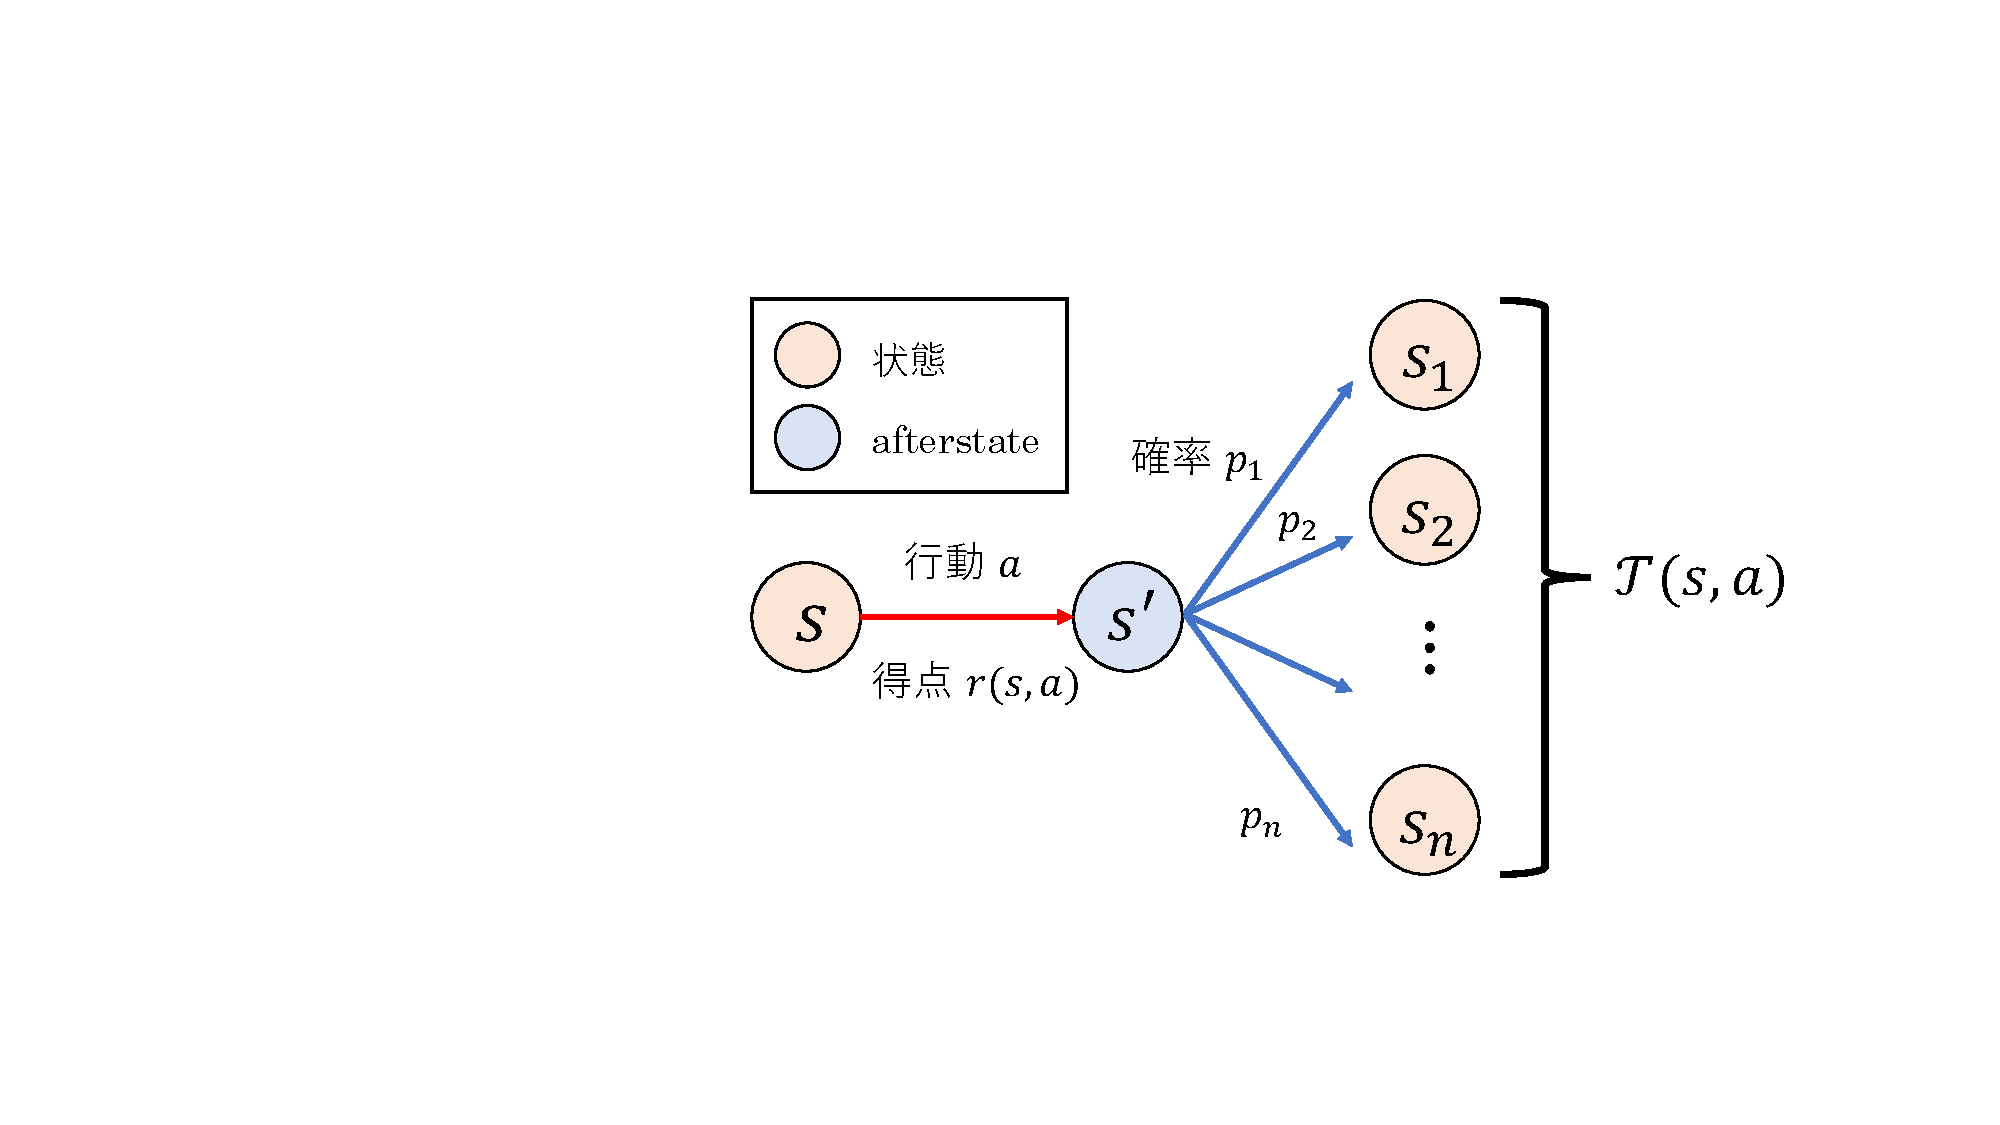
\includegraphics[width=0.6\linewidth{}]{figures/value_function_.pdf}
    \caption{式~\ref{eq:value}の補足図}
    \label{fig:state_afterstate}
\end{figure}

ゲームに現れうるすべての状態の最適価値を計算すれば, 任意の状態において最善手を選ぶことができる.
本稿ではこれを2048の完全解析ということにする.

完全解析をすることで, ゲームの任意の状態の最適価値・最善手を明かし, 最善手を選び続けるプレイヤの戦略を解析することができる.
さらに2048を対象とした強化学習手法の良し悪しを定量的に評価し, より良い手法を提案することができると考えられる.
一方で2048を完全解析することは, そのゲーム木の大きさによる計算コストの観点から現状難しいと考えられる.
そこで本来$4\times4$盤面上で行われる2048のミニゲームとして, 盤面サイズを縮小した2048を完全解析することを考える.

\subsection{盤面サイズが小さな2048の完全解析}
\label{sec:mini2048}
基本的なルールは2048と同じで盤面サイズを$4\times4$から縮小したゲームを完全解析することを考える.
盤面サイズに関わらず, 以下の$2$つのステップを順番に行うことで2048を完全解析することができる.

\begin{enumerate}
    \item ゲームに現れうるすべての状態の列挙
    \item 列挙した状態の価値の計算
\end{enumerate}

\ref{subsec:enumeration}節と~\ref{subsec:calculation}節で具体的な方法について述べる.
なお本節の内容は文献~\cite{3x3_2048}および文献~\cite{4x3_2048}を元に執筆された.

\subsubsection{幅優先探索によるすべての状態の列挙}
\label{subsec:enumeration}
完全解析の第1ステップとして幅優先探索によってゲームに現れうるすべての状態を列挙する.
まず初期状態をキューに詰めて探索を開始する.
キューの先頭の状態$s$を取り出し, $s$から遷移可能な次の状態$s_{\text{next}} \in \mathcal{T}(s)$をキューに追加する.
これをキューが空になるまで繰り返すことで, すべての状態を列挙することができる.

ここで$s_{\text{next}} \in \mathcal{T}(s)$がすでに発見済みであるか確認するために, これまでに発見した状態を管理する集合が必要である.
素朴な方法ではメモリでこれまでに発見した全状態を管理することで行えるが, 状態数が非常に大きな場合にはメモリの容量を超えてしまう.

そこで~\ref{sec:property}節で説明した時刻によってゲーム木を整理する.
時刻$t$の状態は時刻$t+2$か$t+4$の状態にしか遷移しないため, 時刻$t+2$と$t+4$の発見した状態をメモリで管理すれば十分である.
よって時刻が最小の$4$の状態から時刻$2$刻みで順番に列挙を行うことで, ディスクを効率的に活用することができる.
以上を踏まえた疑似コードをAlgorithm~\ref{alg:bfs}に示す.

\begin{algorithm}[tb]
\caption{幅優先探索によるすべての状態の列挙}
\label{alg:bfs}
\begin{algorithmic}[1]
\Function {enumeration}{}
    \For {$t=4$ to $t_{max}$}
        \ForAll {$s_t \in \text{queue}_t$} 
            \ForAll {$s_{t+2} \in \mathcal{T}(s_t)$}
                \State $\text{queue}_{t+2}.\text{push}(s_{t+2})$
            \EndFor
            \ForAll {$s_{t+4} \in \mathcal{T}(s_t)$}
                \State $\text{queue}_{t+4}.\text{push}(s_{t+4})$
            \EndFor
        \EndFor
    \EndFor
\EndFunction
\end{algorithmic}
\end{algorithm}

\subsubsection{後退解析による状態の価値の計算}
\label{subsec:calculation}
\ref{subsec:enumeration}節で列挙した状態の価値を式~\ref{eq:value}に従って計算する.
時刻$t$の状態の価値は, 時刻$t+2$と$t+4$の状態の価値が計算済みであれば計算できる.
よって時刻が最大の状態から順番に走査することで, 効率的にすべての状態の価値を計算できる.
疑似コードをAlgorithm~\ref{alg:calculation}に示す.

\begin{algorithm}[tb]
    \begin{algorithmic}[1]

    \Function {calculation}{$t$}
        \For {$t=t_{max}$ to $4$}
            \State $v(s) = \max_a \left(r(s,a) + \mathbb{E}_{s_\text{next} \in \mathcal{T}(s,a)} v_*(s_\text{next}) \right)$
        \EndFor
        \ForAll {$s_t \in \text{queue}_t$} 
            \ForAll {$s_{t+2} \gets s_t$}
                \State $\text{queue}_{t+2}.\text{push}(s_{t+2})$
            \EndFor
            \If {$element > max$}
                \State $max \gets element$
            \EndIf
        \EndFor
        \State \Return $max$
    \EndFunction
    \end{algorithmic}
    \caption{後退解析による価値計算}
    \label{alg:calculation}
\end{algorithm}

\subsection{実験結果}
$2\times2$盤面から$4\times3$盤面までの2048を完全解析した結果を表~\ref{table: analysis_table}に示す.
\begin{table}[t]
    \centering
    \begin{tabular}{rrr}
        \hline \hline
        盤面サイズ & 状態数 & 初期状態の価値\\ \hline
        $2\times2=4$ & $110$ & $67.6$ \\
        $3\times2=6$ & $21,752$ & $480.9$ \\
        $4\times2=8$ & $4,980,767$ & $2,642.6$ \\
        $3\times3=9$ & $48,713,519$ & $5,469.2$ \\
        $4\times3=12$ & $1,152,817,492,752$ & $50,724.2$ \\
        \hline
    \end{tabular}
    \caption{盤面の大きさと解析結果に関する表}
    \label{table: analysis_table}
\end{table}
盤面サイズが大きくなるに従って指数関数的に状態数は大きくなることが分かる.
また初期状態の価値は, 盤面サイズが$n$マス増える度に$2^n \sim 2^{n+1}$倍になっていることが分かる.
そのため$4\times4$盤面の2048は完全解析を行うには状態数が非常に大きく, 初期状態の価値は約$800,000$点程度ではないかと予想される.

$3\times3$盤面と$4\times3$盤面の2048の各時刻における状態数のグラフを図~\ref{fig:state_afterstate}に示す.
多くのゲームでは進行に従って多様な盤面が存在するため状態数は大きくなり続ける.
一方で2048は盤面が数字タイルで埋まるとゲームオーバーになりやすく, その時刻の状態数は少なくなる.
大きな数字タイルを完成させると盤面上に空きマスが増え, ゲームは再び複雑性を増す.
実際, 図~\ref{fig:state_afterstate}からは$2^n$の前後の時刻で状態数が大きく増減していることが見て取れる.
よって2048はゲームの進行に従って, ゲームの複雑性が増減するという特徴を持つ.
このため任意の時刻における状態数は一定の上限で抑えられ, ~\ref{subsec:enumeration}節と~\ref{subsec:calculation}節で説明した完全解析を実行できる.
\begin{figure}
\vspace{0.2cm}
\begin{subfigure}[T]{0.3\columnwidth}
    \centering
    \includegraphics[width=\columnwidth]{figures/graph_mini_.pdf}
    \caption{$3\times3$盤面の2048}
    \label{fig:graph_mini}
\end{subfigure}
\begin{subfigure}[T]{0.3\columnwidth}
    \centering
    \includegraphics[width=\columnwidth]{figures/graph_mid_.pdf}
    \caption{$4\times3$盤面の2048}
    \label{fig:graph_mid}
\end{subfigure}
\begin{subfigure}[T]{0.3\columnwidth}
    \centering
    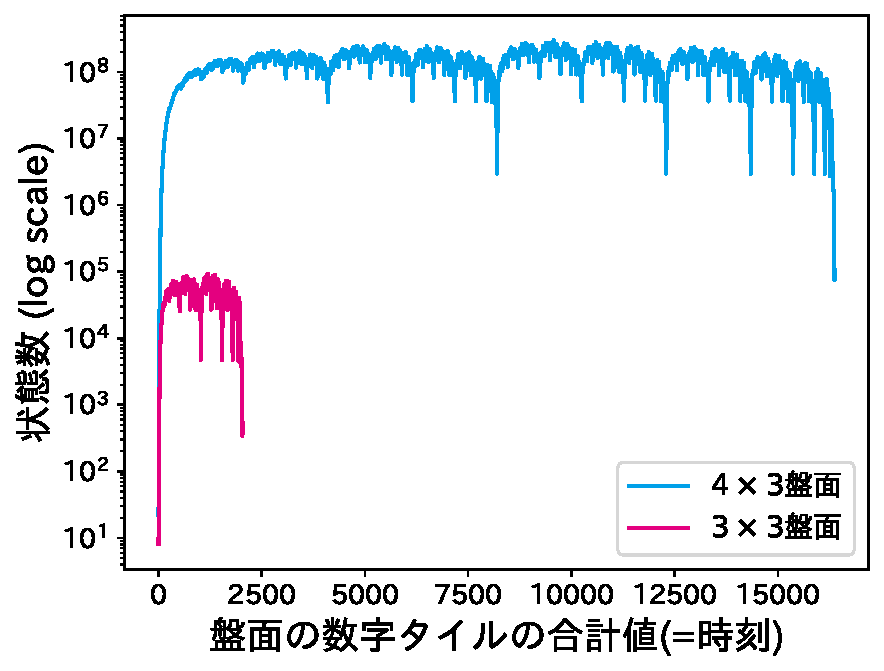
\includegraphics[width=\columnwidth]{figures/graph_compare_mid_mini_.pdf}
    \caption{$3\times3$盤面と$4\times3$盤面の状態数の比較}
    \label{fig:graph_compare_mid_mini_}
\end{subfigure}
\caption{時刻と状態数のグラフ}
\label{fig:time_state_num}
\end{figure}

参考として, $2\times2$盤面の2048のゲーム木全体を図~\ref{fig:game_tree}に示す.
ゲーム木が増大と縮小を繰り返す様子が見て取れる.
\begin{figure}[t]
    \centering
    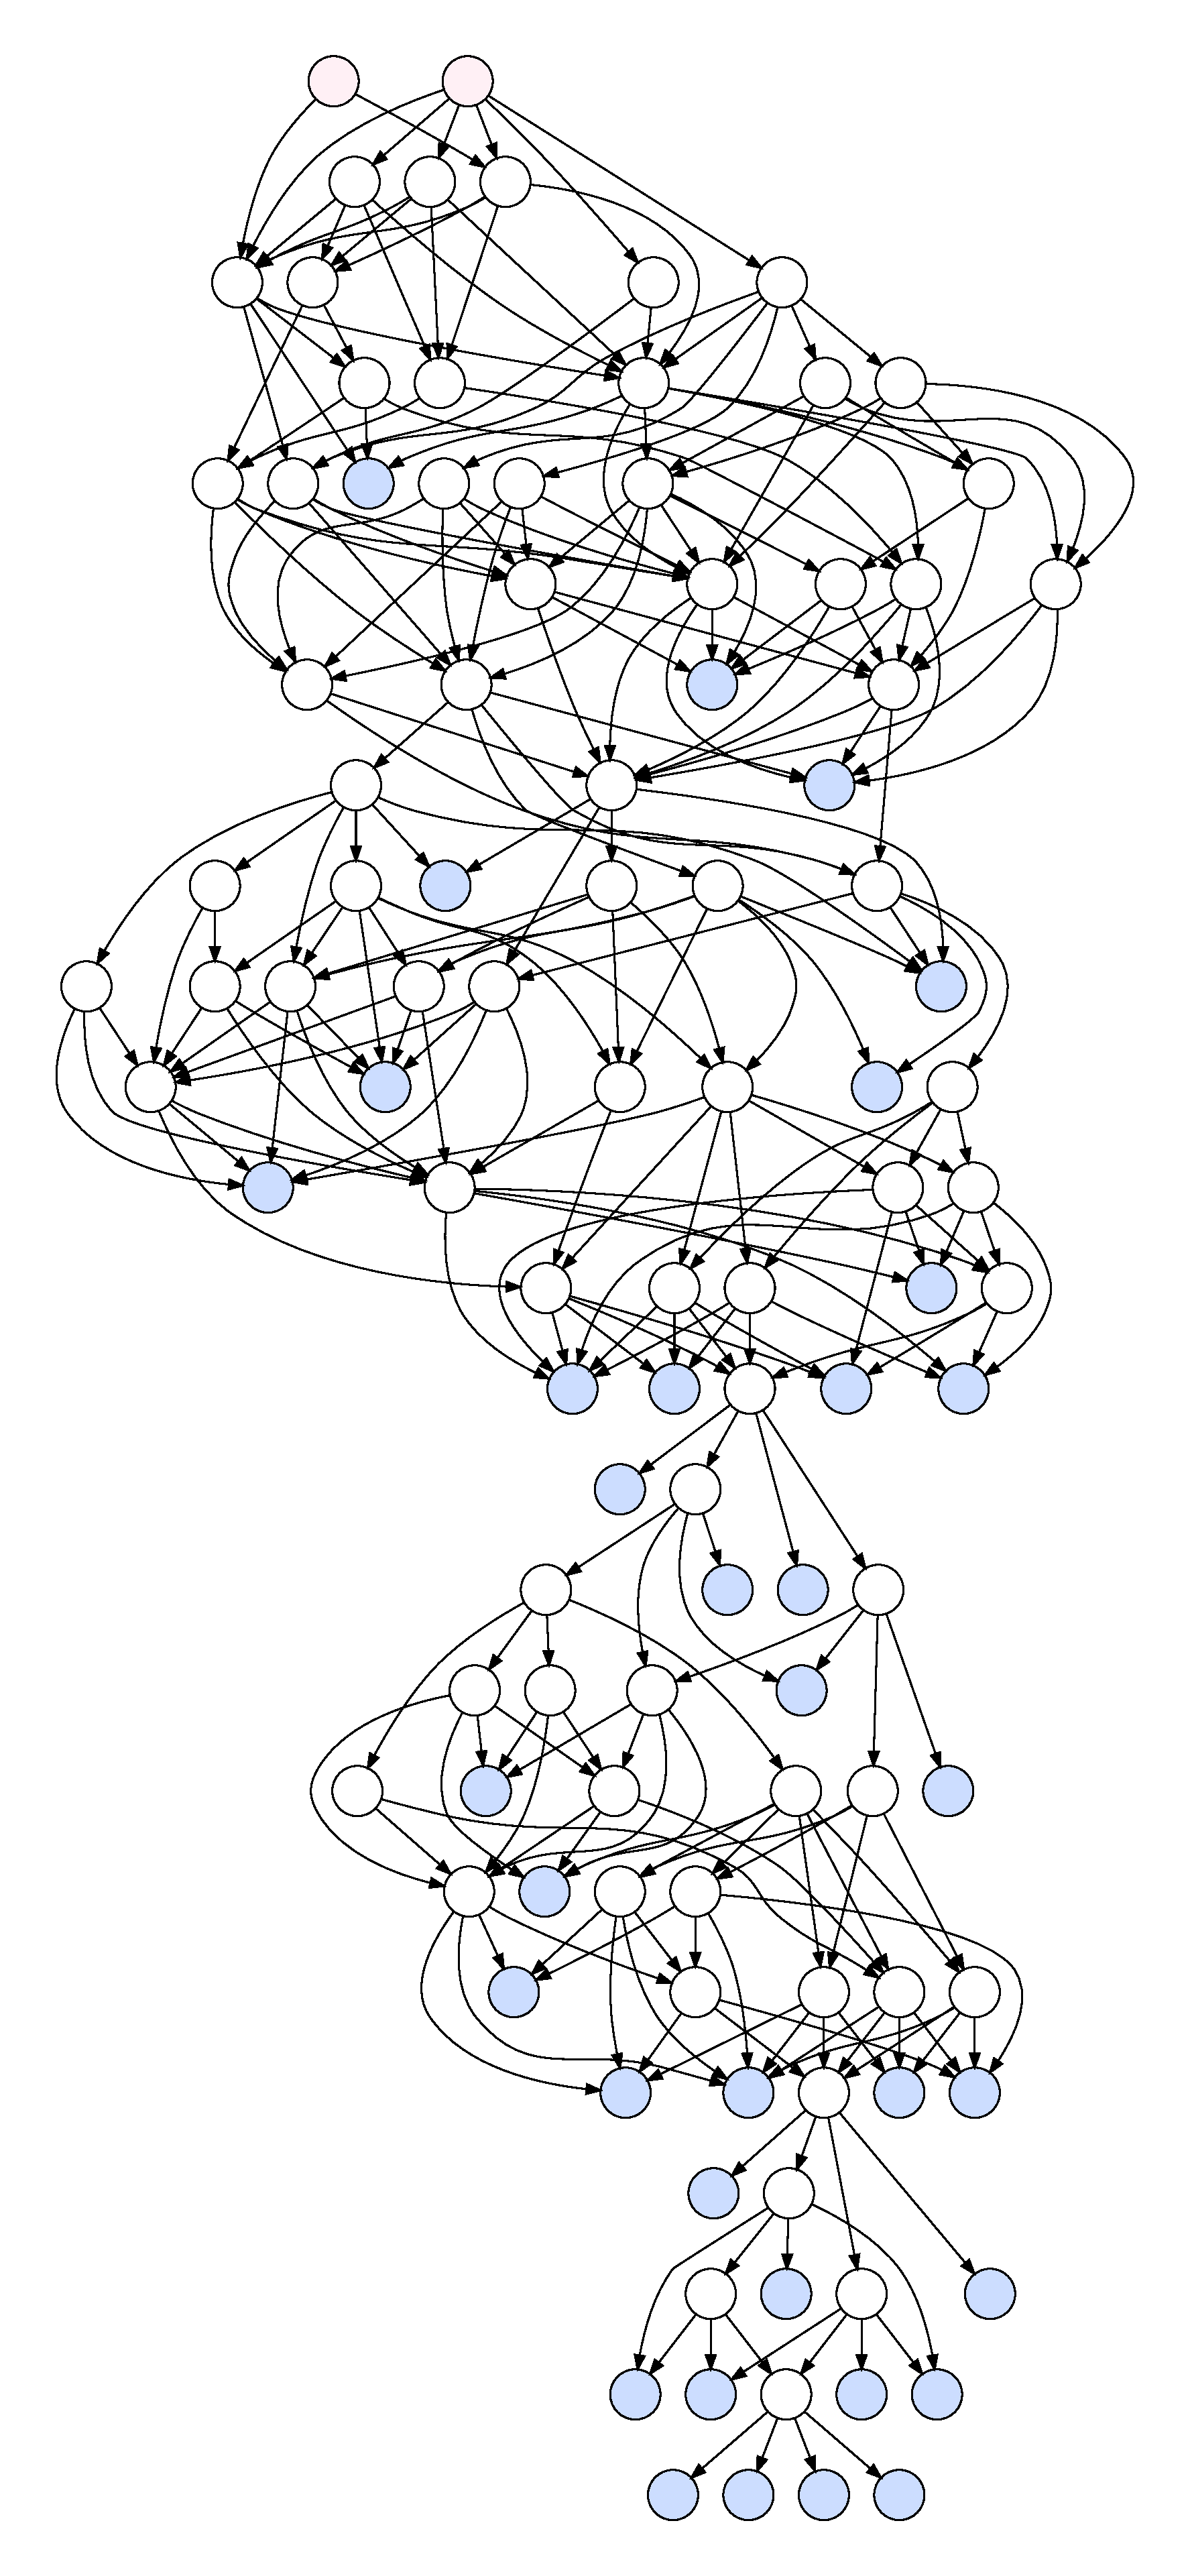
\includegraphics[width=0.7\linewidth{}]{figures/tree.pdf}
    \caption{$2\times2$盤面の2048のゲーム木~(赤色のノードは初期状態, 青色のノードは終了状態)}
    \label{fig:game_tree}
\end{figure}

\section{2048のミニゲームの完全解析と強化学習}
\ref{chap:solving}節では強化学習のベンチマークとしての2048のミニゲームの提案, およびその完全解析を行った.
これらのミニゲームをベンチマークとすることで, 2048の強化学習手法の定量的評価を行うことができる.
これを題材として本研究では, \ref{subsec: stochastic_muzero}節で述べた, 汎用的で2048においても現状最も有力で強化学習手法の$1$つであるStochastic MuZero~\cite{StochasticMuZero}について研究する.
ただしStochastic MuZeroのように, 環境のダイナミクスモデルを学習するには多くの計算資源を要する.
そのため本稿では, 環境のダイナミクスは既知として, 状態を評価する方策・価値ネットワーク, afterstateを評価する価値ネットワークの訓練のみを行う2048-AlphaZeroを考える.
2048-AlphaZeroの学習において, MCTSによるプランニングやニューラルネットワークの学習方法がどのように影響するのかを, 詳細に検証する.
本研究で実験する2048-AlphaZeroのニューラルネットワークは, Resnet~\cite{Resnet}のアーキテクチャによって実装された.
アーキテクチャの詳細は付録~\ref{subsec:nn_impl}に記述した.

\subsection{$3\times3$盤面の2048における強化学習の研究}
本節では$3\times3$盤面の2048を題材として, 2048-AlphaZeroの評価を行う.
$3\times3$盤面の2048ではいずれの実験においても, 図~\ref{fig:nn_arch}のResidual Blockは$5$個, num filtersは$64$のニューラルネットワークを用いた.

2048-AlphaZeroは訓練時と, 訓練後の性能の評価時の両方でMCTSによるプランニングを行う.
\ref{subsubsec:mcts}節で述べたように, MCTSはシミュレーションという単位で実行される.
シミュレーションの回数が大きいほど, 探索は深く正確になる.
以降では訓練時のシミュレーション回数が$n$回, 評価時のシミュレーション回数が$m$回のエージェントを$\text{train-}n,\text{eval-}m$のように表す.
また評価時には$1,000$回のゲームの平均得点を用いる.

\subsubsection{$3\times3$盤面の2048における2048-AlphaZeroの学習}
まず一様ランダムに学習データをサンプルするExperience Replay~(以降Random Experience Replayと表記する)~を用いる手法と, Stochastic MuZeroと同様に予測誤差をpriorityとして重み付けサンプルするPrioritized Experience Replayを用いる手法の$2$つを比較する.
ここでは$3\times{10}^8$回の行動分の学習データを用いて訓練した.
図~\ref{fig:mini2048_alphazero}にそれぞれのエージェント$(\text{いずれもtrain-}100,\text{eval-}100)$の学習の様子を示す.
図中のoptimal value~(最適価値)~とは~\ref{sec:solving}節の完全解析によって得た, $3\times3$盤面の2048の得点の理論値である.
平均得点の最大値は, Random Experience Replayを用いた場合が$5,216.50$点, Prioritized Experience Replayを用いた場合が$5,354.10$点であった.
いずれも学習に従って最適価値に近い得点を獲得するようになるが, Prioritized Experience Replayを使用した方が僅かに点数が伸びる様子が見て取れる.

\subsubsection{MCTSによるプランニングと得点の関係の検証}
次にMCTSによるプランニングが, エージェントの強さにどのように寄与しているかを調べる.
そのために学習時と評価時のMCTSのシミュレーション回数をそれぞれ増減させたときに, エージェントの得点がどう変化するかを実験する.
シミュレーション回数が$10$回, $20$回, $30$回, $50$回, $100$回で訓練したエージェントそれぞれについて, $0 \sim 100$回のシミュレーションで評価した結果を図~\ref{fig:mini2048_alphazero_simulations}に示す.
ただしシミュレーション$0$回のMCTSとは, 状態$s$において方策ネットワークが示す$\pi(\cdot|s)$が最も高い行動を常に選択するものとする.
またいずれの条件においても学習時にはPrioritized Experience Replayを用いる.

訓練時のシミュレーション回数が多いほど, 得点も大きくなることがわかる.
正確なプランニングを行うほど, より良質な学習データを生成することができていると考えられる.
ただしtrain-$50$とtrain-$100$には大きな差はなく, 一定回数以上のシミュレーションを行うことはあまり学習に寄与しないと考えられる.
またニューラルネットワークが十分に訓練されていれば, 評価時にMCTSのシミュレーション数を増減させても得点に大きな変化はない.
特にtrain-$100$は評価時にMCTSを行わなくても, $5,125.01$点と高い平均得点を獲得している.
\begin{figure}
    \begin{subfigure}[T]{0.5\columnwidth}
        \centering
        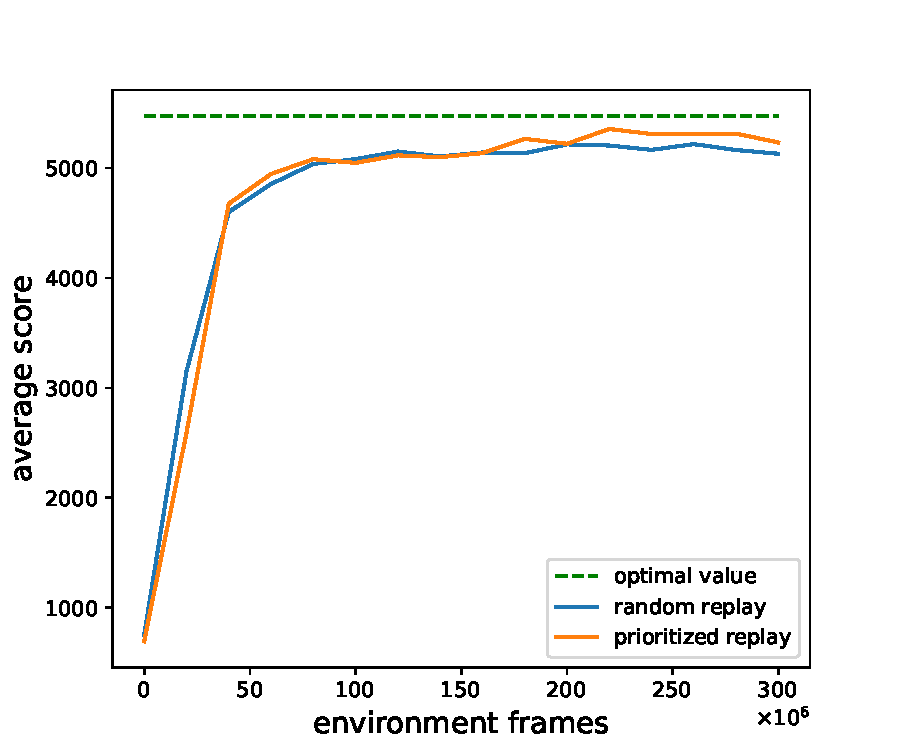
\includegraphics[width=\columnwidth]{figures/alphazero_3x3.pdf}
        \caption{$3\times3$盤面の2048-alphazero}
        \label{fig:mini2048_alphazero}
    \end{subfigure}
    \begin{subfigure}[T]{0.5\columnwidth}
        \centering
        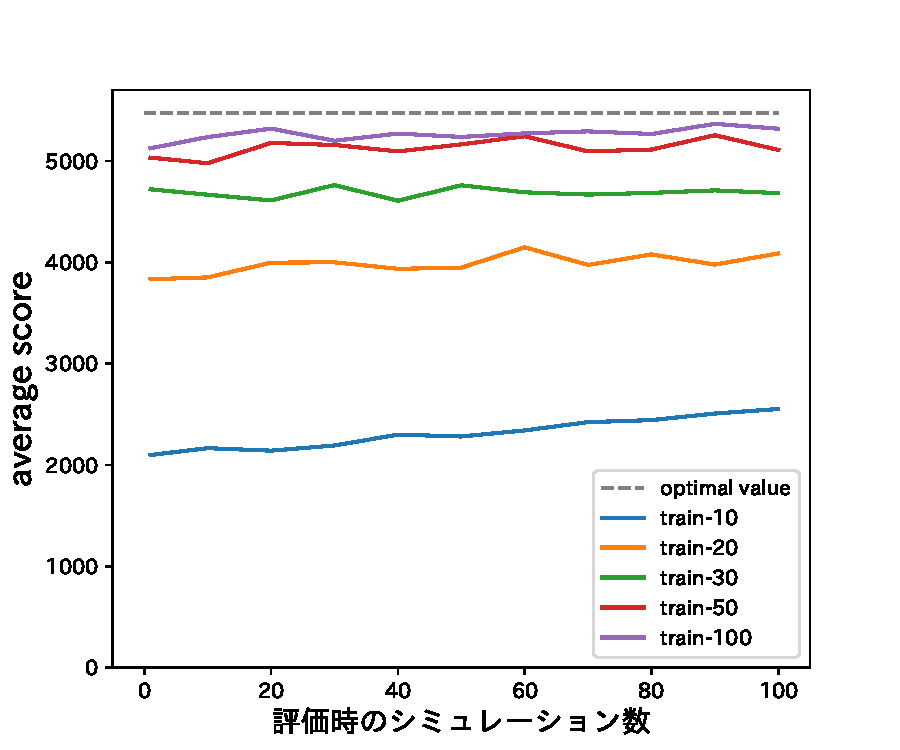
\includegraphics[width=\columnwidth]{figures/3x3_2048_alphazero_simulations.pdf}
        \caption{MCTSのシミュレーション数の増減}
        \label{fig:mini2048_alphazero_simulations}
    \end{subfigure}
\end{figure}

Terauchiら~\cite{Min2048_matsuzaki}は$3\times3$盤面の2048の完全解析結果を題材に, TD-afterstate学習でN-tupleネットワークを訓練したプレイヤを様々な点から評価した.
Terauchiらはパラメータ数が$7.1\times{10}^6$のN-tupleネットワークを$5 \times {10}^8$回の行動分の学習データを用いて訓練したが, 平均$4905.27$点にとどまったと報告している.
一方で本研究で実験した2048-AlphaZeroは, パラメータ数が$568,717$の状態を評価する方策・価値ニューラルネットワークと, パラメータ数$529,417$のafterstateを評価する価値ニューラルネットワークを持つ.
$\text{train-}100,\text{eval-}100$のエージェントは平均$5,354.10$点を達成し, 評価時にMCTSを行わないエージェント$(\text{train-}100,\text{eval-}0)$は平均$5,125.01$点を達成した.
よってTerauchiらのN-tupleネットワーク+TD afterstate学習と比べて2048-AlphaZeroは, 約$7$分の$1$のパラメータ数, $5$分の$3$の学習データを用いて平均得点を上回ることができた.
これらの結果を表~\ref{table:terauchi}にまとめる.
\begin{table}[t]
    \centering
    \begin{tabular}{lrrrr}
        \hline \hline
        手法 & 平均得点 & 訓練時のプランニング & 評価時のプランニング & パラメータ数\\ \hline
        TD afterstate~\cite{Min2048_matsuzaki} & $4,905.27$ & なし & なし & $7,100,000$\\
        2048-AlphaZero & $5,125.01$ & $100$シミュレーション & なし & $1,098,134$\\
        2048-AlphaZero & $5,354.10$ & $100$シミュレーション & $100$シミュレーション & $1,098,134$ \\
        \hline
    \end{tabular}
    \caption{N-tuple+TD afterstate学習と2048-AlphaZeroの比較}
    \label{table:terauchi}
\end{table}

ここまでの実験を踏まえると, 2048-AlphaZeroが優れている要因として以下が考えられる.
\begin{itemize}
    \item ニューラルネットワークの関数近似手法としての優れた汎化性能
    \item 訓練時のMCTSによる良質な学習データの獲得
\end{itemize}
さらなる研究として, ニューラルネットワークを評価関数としてTD-afterstate学習を行う

\subsubsection{完全解析結果を活用した学習が難しい盤面の調査}
\label{subsubsec:db_analize}
ここまでは$3\times3$盤面の2048の最適価値とエージェントの獲得する得点を比較してきた.
本節では完全解析結果のデータベースをさらに活用して, 学習が難しい盤面を調査する.
本研究では盤面上の空きマスの数に着目した.
一般に空きマスの数が少ない盤面は, ゲームオーバーになる可能性が高く正しい行動をとるのが難しい.
そのため正確な価値を推定するように, ニューラルネットワークを学習させるのも難しいと考えられる.

そこで図~\ref{fig:empty_tiles_accuracy}に盤面上の空きマスの数と, それらの盤面におけるエージェントが示す手と最善手との一致率の関係を示す.
また図~\ref{fig:empty_tiles_abs_error}に盤面上の空きマスの数と, それらの盤面におけるエージェントが選んだ行動の価値と最善手の価値の絶対誤差~(ただしエージェントが最善手と異なる行動をとった回数で平均をとる)~の関係を示す.
いずれの実験においてもPrioritized Experience Replayで訓練したtrain-$100$, eval-$100$のエージェントを用いた.
ここでは$1,000$ゲームをプレイする中で現れたすべての状態を対象とした.
2048のルールでは常に盤面上に少なくとも$2$つの数字タイルが存在するため, $3\times3$盤面の2048では空きマスの数の最大値は$7$である.

図~\ref{fig:empty_tiles_accuracy}より空きマスの数が少ないと, エージェントの行動と最善手の一致率が低くなる傾向があることがわかる.
また図~\ref{fig:empty_tiles_abs_error}より空きマスの数が少ないほど, エージェントの行動価値と最善手の価値の絶対誤差は大きいことがわかる.
よって学習を効率化させるために, 空きマスが少ないデータを優先的に学習に使用するような, Prioritized Experience Replayを使用することが考えられる.
ただし$3\times3$盤面の2048においては, すでにエージェントの得点が最適価値に十分近づいているため, $4\times3$盤面の2048で実験することにする.
\begin{figure}
    \begin{subfigure}[T]{0.5\columnwidth}
        \centering
        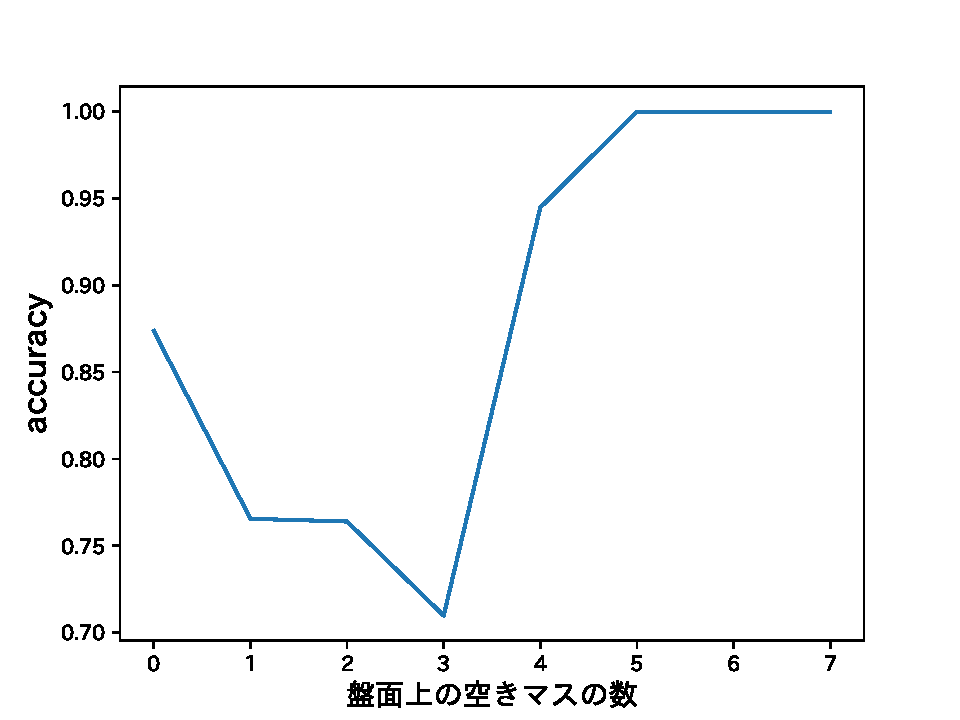
\includegraphics[width=\columnwidth]{figures/empty_tiles_accuracy.pdf}
        \caption{盤面上の空きマスの数と最善手との一致率}
        \label{fig:empty_tiles_accuracy}
    \end{subfigure}
    \begin{subfigure}[T]{0.5\columnwidth}
        \centering
        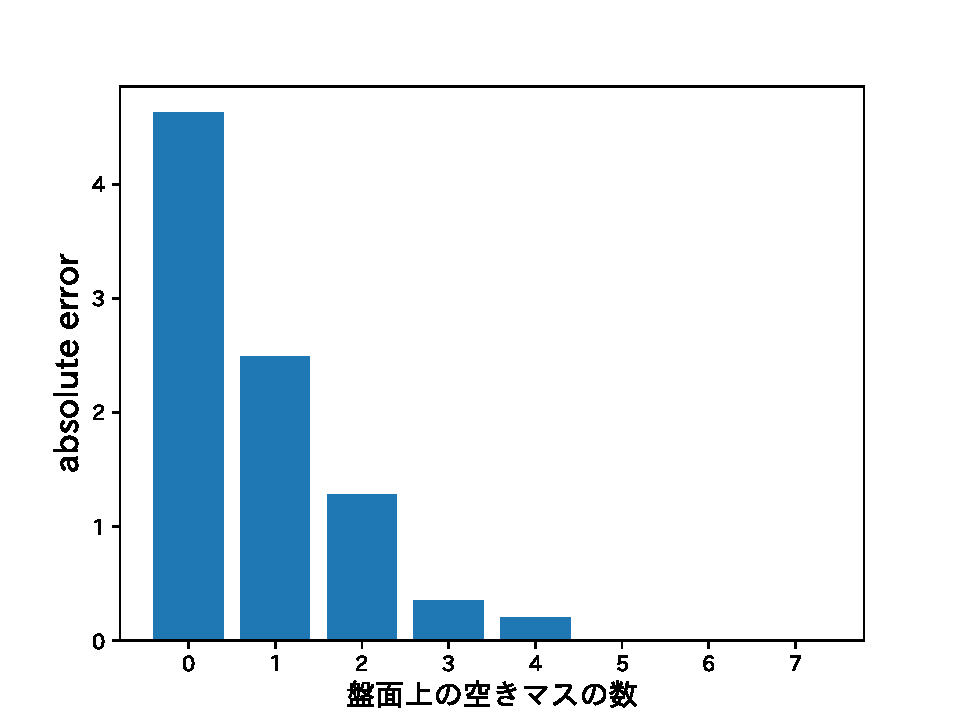
\includegraphics[width=\columnwidth]{figures/empty_tiles_abs_error.pdf}
        \caption{最善手の価値とエージェントが選んだ行動の価値の絶対誤差}
        \label{fig:empty_tiles_abs_error}
    \end{subfigure}
\end{figure}

\subsection{$4\times3$盤面の2048と2048-AlphaZero}
$3\times3$盤面の2048は状態数が比較的少ないため, データベースが軽量でデータを参照しやすい利点がある.
そのため強化学習手法の一手一手の詳細な分析を行うのに適している環境といえる.
実際,\ref{subsubsec:db_analize}節ではデータベースを活用して, エージェントの一手ごとの行動について評価を行った.
一方で図~\ref{fig:mini2048_alphazero}が示すように, $3\times3$盤面の2048では学習したエージェントは得点が最適価値に十分近づいている.
そのため一定以上の性能を持つエージェントを比較するために適しているとは言えない.
よって本節では, より難易度の高い$4\times3$盤面の2048において, 2048-AlphaZeroを評価する.

$3\times3$盤面の実験ではResidual Blockが$5$個のニューラルネットワークのみを用いたが, $4\times3$盤面の実験では, これに加えてより大きな$10$個のニューラルネットワークでも実験を行う.
さらに~\ref{subsubsec:db_analize}節で述べた, 空きマスの少ない盤面データが優先的に学習に使われるようなPrioritized Experience Replayを使用する実験を行う.
具体的には盤面上の空きマスの数を$n$とすると, priorityを$\frac{1}{n}$とする~(ただし$n=0$のときはprioriry$=0.5$とした).
priorityは$1$回学習に使用されるたびに, $0.5$倍に更新する.

図~\ref{fig:mid2048_alphazero}にこれらの手法の実験結果を示す.
実験では$10$ Residual Blockを, Stochastic MuZeroと同様に予測誤差をpriorityとするPrioritized Experience Replayを用いて訓練した手法が最も高得点を獲得した.
空きマスが少ない盤面データを優先的に学習させる手法~(図中のempty tiles replay)~は, 期待に反して他の手法と比べて効率的に学習が進むことはなかった.
全体として, 大きなサイズのニューラルネットワーク
またエージェントの得点は, 学習序盤に急激に伸びた後は緩やかに上昇することが見て取れる.
\begin{figure}[t]
    \centering
    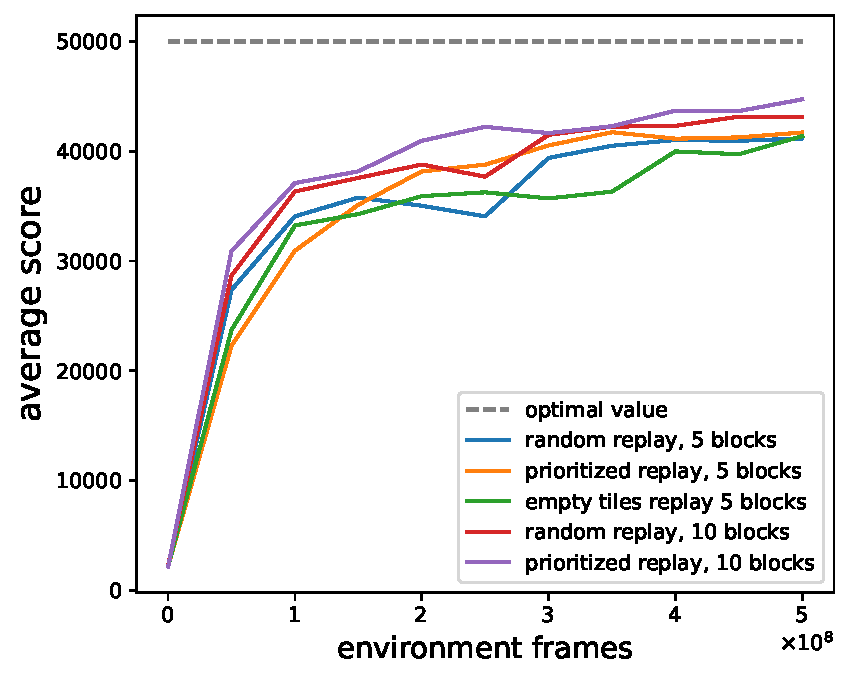
\includegraphics[width=0.6\linewidth{}]{figures/alphazero_4x3.pdf}
    \caption{$4\times3$盤面の2048-alphazero}
    \label{fig:mid2048_alphazero}
\end{figure}  

よってここまでの実験から2048の強化学習手法には以下の要素が重要だと考えられる.

\ref{sec:solving_impl}節で述べるように, $4\times3$盤面の2048の完全解析結果のデータベースは非常に大きく, データの参照などに現状時間を要する.
そのため本稿では,\ref{subsubsec:db_analize}節で$3\times3$盤面の2048で行ったような一手一手の細かい分析を行うことができなかった.
これは簡潔データ構造を用いることで改善することができると考えられる.
データベースの簡潔データ構造化, およびそれを用いた$4\times3$盤面の2048における強化学習手法の詳細な分析は製本版までの課題としたい.

\subsection{$4\times4$盤面の2048と2048-AlphaZero}
これまでのミニゲームでの実験を通して得た知見を踏まえて, オリジナルの$4\times4$盤面の2048で実験を行う.
ただし現状十分な実験を行えていないため, 製本版の提出時に実験結果を記載する.